%%%%%%%%%%%%%%%%%%%%%%%%%%%%%%%%%%%%%%%%%
% Short Sectioned Assignment LaTeX Template Version 1.0 (5/5/12)
% This template has been downloaded from: http://www.LaTeXTemplates.com
% Original author:  Frits Wenneker (http://www.howtotex.com)
% License: CC BY-NC-SA 3.0 (http://creativecommons.org/licenses/by-nc-sa/3.0/)
%%%%%%%%%%%%%%%%%%%%%%%%%%%%%%%%%%%%%%%%%

%----------------------------------------------------------------------------------------
%	PACKAGES AND OTHER DOCUMENT CONFIGURATIONS
%----------------------------------------------------------------------------------------

\documentclass[paper=a4, fontsize=11pt]{scrartcl} % A4 paper and 11pt font size

% ---- Entrada y salida de texto -----

\usepackage[T1]{fontenc} % Use 8-bit encoding that has 256 glyphs
\usepackage[utf8]{inputenc}
%\usepackage{fourier} % Use the Adobe Utopia font for the document - comment this line to return to the LaTeX default

% ---- Idioma --------

\usepackage[spanish, es-tabla]{babel} % Selecciona el español para palabras introducidas automáticamente, p.ej. "septiembre" en la fecha y especifica que se use la palabra Tabla en vez de Cuadro

% ---- Otros paquetes ----

\usepackage{url} % ,href} %para incluir URLs e hipervínculos dentro del texto (aunque hay que instalar href)
\usepackage{amsmath,amsfonts,amsthm} % Math packages
%\usepackage{graphics,graphicx, floatrow} %para incluir imágenes y notas en las imágenes
\usepackage{graphics,graphicx, float} %para incluir imágenes y colocarlas

% Para hacer tablas comlejas
%\usepackage{multirow}
%\usepackage{threeparttable}

%\usepackage{sectsty} % Allows customizing section commands
%\allsectionsfont{\centering \normalfont\scshape} % Make all sections centered, the default font and small caps

\usepackage{fancyhdr} % Custom headers and footers
\pagestyle{fancyplain} % Makes all pages in the document conform to the custom headers and footers
\fancyhead{} % No page header - if you want one, create it in the same way as the footers below
\fancyfoot[L]{} % Empty left footer
\fancyfoot[C]{} % Empty center footer
\fancyfoot[R]{} % Page numbering for right footer
\renewcommand{\headrulewidth}{0pt} % Remove header underlines
\renewcommand{\footrulewidth}{0pt} % Remove footer underlines
\setlength{\headheight}{13.6pt} % Customize the height of the header

\numberwithin{equation}{section} % Number equations within sections (i.e. 1.1, 1.2, 2.1, 2.2 instead of 1, 2, 3, 4)
\numberwithin{figure}{section} % Number figures within sections (i.e. 1.1, 1.2, 2.1, 2.2 instead of 1, 2, 3, 4)
\numberwithin{table}{section} % Number tables within sections (i.e. 1.1, 1.2, 2.1, 2.2 instead of 1, 2, 3, 4)

\setlength\parindent{0pt} % Removes all indentation from paragraphs - comment this line for an assignment with lots of text

\newcommand{\horrule}[1]{\rule{\linewidth}{#1}} % Create horizontal rule command with 1 argument of height


\usepackage{hyperref}
\usepackage{listings}
\usepackage{xcolor}
\usepackage{caption}
\usepackage{subcaption}
\usepackage{lmodern}
\usepackage{graphicx}
\usepackage{biblatex}
\usepackage{array}
\usepackage{wrapfig}

\definecolor{codegreen}{rgb}{0,0.6,0}
\definecolor{codegray}{rgb}{0.5,0.5,0.5}
\definecolor{codepurple}{rgb}{0.58,0,0.82}
\definecolor{backcolour}{rgb}{0.95,0.95,0.92}

\newcolumntype{C}[1]{>{\centering\arraybackslash}p{#1}}
\newcolumntype{L}[1]{>{\raggedright\arraybackslash}p{#1}}
\newcolumntype{R}[1]{>{\raggedleft\arraybackslash}p{#1}}

\lstdefinestyle{mystyle}{
    backgroundcolor=\color{backcolour},   
    commentstyle=\color{codegreen},
    keywordstyle=\color{magenta},
    numberstyle=\tiny\color{codegray},
    stringstyle=\color{codepurple},
    basicstyle=\ttfamily\footnotesize,
    breakatwhitespace=false,         
    breaklines=true,                 
    captionpos=b,                    
    keepspaces=true,                 
    numbers=left,                    
    numbersep=5pt,                  
    showspaces=false,                
    showstringspaces=false,
    showtabs=false,                  
    tabsize=2
}


\title{	
\normalfont \normalsize 
\textsc{\textbf{Metaheurística grupo 2 (2021-2022)} \\ Grado en Ingeniería Informática \\ Universidad de Granada} \\ [25pt] % Your university, school and/or department name(s)
\horrule{0.5pt} \\[0.4cm] % Thin top horizontal rule
\huge Práctica 1 \\
Mínima dispersión diferencial \\ % The assignment title
\horrule{2pt} \\[0.5cm] % Thick bottom horizontal rule
}

\author{José María Ramírez González\\\href{mailto:jmramirez@correo.ugr.es}{jmramirez@correo.ugr.es}\\32899118X} % Nombre y apellidos

\date{\normalsize\today} % Incluye la fecha actual

\begin{document}

\maketitle % Muestra el Título

\newpage %inserta un salto de página

\tableofcontents % para generar el índice de contenidos

\listoffigures

\lstlistoflistings

\newpage

\section{Descripción del problema}

El problema escogido es el conocido como \textit{mínima dispersión diferencial} o \textit{minimun differential dispersion} en inglés.

Este problema trata de intentar minimizar la dispersión entre un subconjunto $M$ de elementos de un conjunto $C$. Es un problema \textbf{NP-completo}, por lo que resulta inviable resolverlo de manera óptima en un tiempo decente en casos donde $|C|$ o $|M|$ sean grandes.

Nuestro objetivo es encontrar $M \subset C$, y se nos proporcionarán varios casos, cada uno con un $C$ y un $m =|M|$.
En cada caso nos dan, además, la distancia de un elemento al resto de ellos, tal que podamos calcular el \textit{$\Delta$-value} de cada elemento como $\displaystyle \Delta \text{-value}_i = \sum_{j \in M}d_{ij}\quad \forall \, i \in M$, donde $d_{ij}$ es la distancia del elemento $i$ al elemento $j$.

Para calcular la dispersión, realizamos el siguiente cálculo $disp = max(\Delta\text{-value})-min(\Delta\text{-value})$. Esa sería la dispersión asociada a una posible solución $M$, el máximo de sus $\Delta$-values menos el mínimo de ellos. Así pues, nuestro función a minimizar es esa.

Es importante destacar, que la dispersión de cada conjunto solución $M$ depende de cada uno de los elementos $w \in M$ y que, cambiando tan solo uno de ellos, esta puede cambiar radicalmente.

\newpage
\section{Elementos comunes empleados en la resolución del problema}
Para resolver este problema, hemos implementado dos algoritmos distintos:
\begin{itemize}
\item Un algoritmo \textbf{Greedy}.
\item Un algoritmo de \textbf{Búsqueda local}.
\end{itemize}

Más adelante estudiaremos estos algoritmos, pero antes, vamos a comentar algunos elementos comunes a ambos.

\subsection{Representación de los datos}

Los datos de entrada se nos proporcionan en un fichero con la estructura que podemos apreciar en el listing \ref{lst:estructuraFicheros}.

\begin{lstlisting}[frame=single,caption={Estructura de los ficheros proporcionados},label=lst:estructuraFicheros, captionpos=b]
n m
0 1 value
0 2 value
...
n-2 n-1 value
\end{lstlisting}

Donde $m = |M|$, $n = |C|$ y \textit{value} es el coste de ir de la posición que aparece primero a la posición que aparece en segundo lugar.

En nuestro caso, guardaremos esta información en forma de matriz cuadrada $n \times n$, donde rellenamos el triangulo superior y el inferior, para no tener que comprobar índices, y dejaremos 0s en la diagonal principal.

El funcionamiento general sería el que observamos en el listing \ref{lst:funcionamientoLeerDatos}.

\begin{lstlisting}[frame=single, caption={Generalización de la lectura de los datos},label=lst:funcionamientoLeerDatos, captionpos=b]
archivo = open(archivoConDatos)
n, m = archivo.get(0,1)

# Nueva matriz de tam n*n inicializada a 0
matriz = nuevaMatriz(n x n, 0)

for linea in archivo:
    pos1 = linea[0]
    pos2 = linea[1]
    valor = linea[2]
    matriz[pos1][pos2] = valor
    matriz[pos2][pos1] = valor
\end{lstlisting}


\subsection{Función objetivo}

Nuestro objetivo es minimizar la dispersión, calculada como $disp = max(\Delta\text{-value})-min(\Delta\text{-value})$.

Para ahorrar tiempo de procesado, no vamos a calcular los $\Delta\text{-value}$ de cada conjunto solución, si no que iremos recalculando por cada elemento que incluyamos (versión \textit{greedy}) o cambiemos (versión \textit{búsqueda local}) en el conjunto solución.
Es decir, si antes teníamos $X \ \Delta\text{-values}$, ahora que hemos cambiado/añadido este elemento, modificamos cada $\Delta\text{-value} \in X$ según corresponda.

Esto acelerará los cálculos al no tener que calcular todos los valores de 0.

Así pues, cambiar un elemento tal que la nueva dispersión $\displaystyle disp' < disp$ o añadir uno nuevo tal que $disp'$ sea lo más cercana a $disp$ posible, es decir, no aumente mucho la dispersión.

En la figura \ref{fig:fObjetivo}, tenemos los pseudocódigos para ambos casos del funcionamiento de la función objetivo.

\begin{figure}[H]
    \centering
    \begin{subfigure}[b]{0.49\textwidth}
\begin{lstlisting}[caption={Versión greedy}, captionpos=b]
hasta que |Sol|=m:
    para elem en elementos:
        si elem no en Sol:
            calc. valor
    Sol += elem con min(valor)
\end{lstlisting}
    \end{subfigure}
    \begin{subfigure}[b]{0.49\textwidth}
\begin{lstlisting}[caption={Versión búsqueda local}, captionpos=b]
hasta que no varie Sol, para todos elems:
    cambiar elem i opor elem j
    calcular nuevo valor
    si nuevo valor < valor ant:
        aceptar cambio
\end{lstlisting}
    \end{subfigure}
    
\caption{Función objetivo}
\label{fig:fObjetivo}

\end{figure}


\subsection{Selección de los datos de entrada}

Para seleccionar los datos de entrada, hacemos uso de la librería \textit{os} con la que, introduciendo el nombre de la carpeta donde tenemos todos los archivos con los datos de entrada, nos leerá los nombres de los mismos.

Una vez tengamos los nombres, los ordenamos basándonos en los nombres de los mismos con una función que hemos creado y pasamos a ejecutar un bucle que realiza ambos algoritmos (\textit{búsqueda local} y \textit{greedy}) para cada uno.

Podemos encontrar el pseudocódigo en el listing \ref{lst:lecturaArchivos}.

\begin{lstlisting}[frame=single, caption={Versión búsqueda local}, captionpos=b, label=lst:lecturaArchivos]
archivos = leerCarpeta(nombreCarpeta)
ordenar(archivos)
para cada archivo en archivos:
    leer(archivo)
    Ejecutar algoritmos
\end{lstlisting}


\subsection{Aleatoriedad en los algoritmos}

Como se nos explica en el guión de la práctica, necesitamos incluir cierta aleatoriedad en los algoritmos.

Para controlarla y que los experimentos realizados puedan repetirse, hemos establecido las semillas previamente, que son similares para cada ejecución de cada algoritmo, es decir, para cada conjunto de datos, tenemos 5 (en nuestro caso) semillas, una para ejecución que realizaremos.

Así pues, para cada archivo que leemos, realizamos \textbf{5} iteraciones con los dos algoritmos, cada una con una semilla distinta.

La aleatoriedad se incluye de forma similar en cada algoritmo, siendo esta necesaria tan solo al comienzo del mismo.

En el caso del algoritmo \textit{greedy}, se usa para seleccionar los 2 elementos iniciales con los que comenzaremos la ejecución.

En el caso del algoritmo de \textit{búsqueda local}, se usa para seleccionar el conjunto solución inicial, del que partiremos para ejecutar el algoritmo, y para barajar el conjunto de elementos que no están en el conjunto solución.

\subsection{Medición del tiempo de ejecución}

Para medir los tiempos de ejecución de cada algoritmo, hemos hecho uso de la librería \textit{time}, la cual nos proporciona el tiempo de CPU que tarda en ejecutarse una determinada parte del código con una implementación similar a la del listing \ref{lst:tiempoCPU}.

\begin{lstlisting}[frame=single, caption={Tiempo de ejecución de un programa}, captionpos=b, label=lst:tiempoCPU]
tiempoinicio = tiempoActual()

...
#Ejecucion del algoritmo
...

tiempoFinal = tiempoACtual()
tiempoEjecucion = tiempoFinal - tiempoInicio
\end{lstlisting}

\newpage

\section{Algoritmo greedy}

Como primer algoritmo, hemos implementado uno de tipo voraz, este deberá ofrecer tiempos de ejecución realmente bajos, pero también soluciones que son, en algunos casos, bastante alejadas de la óptima.

El funcionamiento general por el que hemos optado consiste en seleccionar dos elementos aleatorios de la muestra e ir, a partir de estos dos, añadiendo nuevos elementos que nos garanticen la menor dispersión posible.
Una vez hayamos llegado al tamaño $m$ que se nos pide, terminamos la ejecución.

\subsection{Funcionamiento del algoritmo}

El algoritmo vamos a ejecutarlo en bucle, de forma que se ejecute hasta que tenemos $m$ elementos en la solución, como hemos señalado anteriormente. Por cada iteración del mismo, calcularemos los $\Delta$-values con los elementos que llevemos en la solución e iteraremos por todos aquellos elementos que no están en nuestra solución actual, comparando que pasaría con la dispersión si añadimos cada elemento a la solución actual, quedándonos al final con aquel que aumente lo menos posible la dispersión.

Podemos ver el pseudocódigo del algoritmo en el listing \ref{lst:funcionamientoGreedy}.

\begin{lstlisting}[frame=single, caption={Funcionamiento del algoritmo greedy}, captionpos=b, label=lst:funcionamientoGreedy]
Hasta que longitud(Sol) distinto de m:
    calcular Delta-values
    
    por cada elemento disponible que no este en Sol:
        posibleSolucion = Sol + elemento
        posiblesDelta = actualizarDelta(posibleSolucion)
        
        si dispersion(posiblesDelta) < minimoActual:
            minimoActual = dispersion(posiblesDelta)
            elementoSeleccionado = elemento
    
    Sol += elementoSeleccionado
\end{lstlisting}

En lo referente a la implementación, no contamos con funciones como sería \textit{dispersión} o \textit{actualizarDelta}, y lo hemos implementado directamente en el bucle, ya que es una operación que no resulta demasiado costosa y no ocupa un tamaño de código excesivo, no obstante, se podrían declarar como función si se quisiera.

Una vez que acabemos el bucle, puesto que no guardamos los $\Delta$-values actualizados cuando añadimos el elemento, sería necesario recalcularlos todos. Se podría guardar este valor durante la ejecución del bucle, pero la mejora en tiempo de ejecución sería despreciable.

\subsection{Orden de tiempo del algoritmo}

En base al listing \ref{lst:funcionamientoGreedy}, si lo observamos con detalle, podemos destacar \textbf{dos} bucles importantes en el mismo:

\begin{itemize}
\item Un bucle \textit{while}.
\item Un bucle \textit{for}.
\end{itemize}

A grandes rasgos, esto nos daría un tiempo teórico del orden $\displaystyle O \Big( m\cdot(n-m) \Big)$, no obstante, más adelante haremos un estudio empírico del mismo para verificar estos tiempo de ejecución.

\newpage

\section{Algoritmo de búsqueda local}

Como se nos pide, hemos llevado a cabo también un algoritmo de búsqueda local, que debería ofrecer unos resultados más cercanos al óptimo teniendo un impacto algo mayor en el tiempo de ejecución en comparación con el voraz, pero sin resultar extremadamente lento.

\subsection{Funcionamiento del algoritmo}

En este caso, lo que realizaremos será comenzar con una solución aleatoria, e ir explorando esta solución realizando cambios entre elementos con aquellos que no formen parte de esta para mejorar el resultado. Estos cambios entre elementos se realizan uno a uno, no siendo posible intercambiar dos o más elementos a la vez.

Podemos verlo como explorar un árbol hasta llegar a un nodo hoja desde el que no podemos mejorar más la solución. En este árbol, cada nodo tendrá $m \cdot n$ padres y $m \cdot n$ hijos, siendo cada uno de ellos el resultado de intercambiar un elemento concreto por otro. Importante destacar que el padre de un nodo, también es hijo del mismo, ya que sería el resultado de volver a intercambiar los mismos elementos.

Una vez que pasemos a un hijo, no podremos volver al padre, es decir, no podemos realizar \textit{backtracking}, resultando en un algoritmo del tipo ``el primer mejor'', ya que una vez que encontremos un hijo mejor que el padre, pasaremos a ese directamente.

A su vez, limitaremos la ejecución del algoritmo a un máximo de 100000 iteraciones, para evitar un bucle infinito.

Podemos ver el pseudocódigo del mismo, que corresponde a nuestra implementación, en el listing \ref{lst:funcionamientoBL}.
\newpage
\begin{lstlisting}[frame=single, caption={Funcionamiento del de búsqueda local}, captionpos=b, label=lst:funcionamientoBL]
Barajar(posiblesOpciones)
Sol = Seleccionar(m, posiblesOpciones)

Mientras cambie y no superemos las maximas iteraciones:
    Barajar(posiblesOpciones):
    Para cada elementoSol en Sol:
        Para cada elemento en posibles opciones:
            nuevaSol = Int(Sol, elementoSol, elemento)
            nuevoCoste = RecalcularCoste(Sol, elementoSol, elemento)
            
            Si nuevoCoste menor que costeAnterior:
                Sol = nuevaSol
                costeAnterior = nuevoCoste
                posiblesOpciones.quitar(elemento)
                posiblesOpciones.meter(elementoSol)
                SalirBuclesFor
                
            iteracion += 1

\end{lstlisting}

La función \textit{Int} que observamos en el listing anterior se usa para intercambiar el elemento \textit{elementoSol}, presente en \textit{Sol} por el elemento \textit{elemento}.

La función \textit{RecalcularCoste} no se encuentra implementada en nuestro programa, pero consta de varias líneas que lo que hacen es actualizar los costes de la nueva solución tan sólo realizando los cambios necesarios en los valores, resultando en una función bastante eficiente a nivel de tiempo.

\subsection{Orden de tiempo del algoritmo}

En base al listing \ref{lst:funcionamientoBL}, si lo observamos con detalle, podemos destacar \textbf{tres} bucles importantes en el mismo:

\begin{itemize}
\item Un bucle \textit{while}.
\item Dos bucle \textit{for}.
\end{itemize}

A grandes rasgos, esto nos daría un tiempo teórico del orden $\displaystyle O \Big( 100000 \cdot m \cdot (n-m) \Big)$, no obstante, más adelante haremos un estudio empírico del mismo para verificar estos tiempo de ejecución.


\newpage

\section{Desarrollo y uso del software}

En esta sección vamos a comentar cómo hemos desarrollado el software para la práctica, a la vez que indicaremos como ejecutar el mismo.

\subsection{Implementación}

A la hora de implementar ambos algoritmos, hemos optados por usar \textit{Python} debido a la sencillez del código, la simplicidad de uso, unos tiempos de ejecución decentes (más lentos que si usamos un lenguaje como \textit{C}, pero correctos para este tipo de software) y, lo más importante, las librerías disponibles y el fácil manejo de tipos de datos como las listas y las matrices.

Ambos algoritmos están escritos en el mismo programa, por lo que no nos tendremos que preocupar de ejecutar varios archivos.

Junto con la memoria, incluiremos un archivo de requisitos en formato \textit{.txt}, de forma que se pueda hacer uso de \textit{pip} para instalar las librerías pertinentes, aunque a excepción de \textit{NumPy}, las otras que usamos vienen instaladas por defecto, por lo que sólo tendríamos que instalar esta.

Es importante destacar que el ejecutable escribe a disco, dejando los resultados en un archivo de nombre \textit{results.txt}, con el formato que se observa en el listing \ref{lst:formatoResults}.

\begin{lstlisting}[frame=single, caption={Formato del archivo results.txt}, captionpos=b, label=lst:formatoResults]
Greedy y BL: DispMedia DispMin DispMax TMedio TMin TMax
Para cada archivo en orden

Ejemplo:

45 25 60 0.7 0.45 1.1 45 25 60 0.7 0.45 1.1
45 25 60 0.7 0.45 1.1 45 25 60 0.7 0.45 1.1
45 25 60 0.7 0.45 1.1 45 25 60 0.7 0.45 1.1

\end{lstlisting}

\subsection{Manual de uso}

Para ejecutar correctamente el ejecutable (\textit{.py}), tan sólo tenemos que hacer uso de \textit{pip} para instalar los requisitos proporcionados en el archivo \textit{requirements.txt}
con el comando \texttt{pip install -r /path/to/requirements.txt}.

Una vez instalado, tenemos que asegurarnos de comprobar que tenemos en una carpeta localizada los archivos a leer y \textbf{solo} esos archivos, ya que el programa no realiza comprobación sobre los archivos que lee. Esta carpeta se la pasaremos por parámetros al momento de ejecución.

Ahora podemos pasar a ejecutar el archivo con el comando \texttt{python3 <nombreArchivo>.py <ruta carpeta datos>}.

Podremos observar los resultado en tiempo real de los valores medios de tiempo y dispersión para ambos algoritmos y, si queremos también los valores mínimo y máximo de tiempo y dispersión, podremos abrir el archivo \textit{resulsts.txt} que aparecerá en el mismo directorio del ejecutable.

Las semillas para controlar la aleatoriedad vienen definidas en el propio código en una variable llamada \textit{seeds}\footnote{Las semillas utilizadas son 19102001 ,20102001, 19112001, 19102002 y 21112001}, que se encuentra en la línea 46. Si cambiamos los valores, obtendremos resultados diferentes a la hora de ejecutar el programa, y si queremos optar por no utilizar semillas, podemos comentar la línea 46 y la línea 67, siendo esta última la que fija la semilla a utilizar.
\newpage

\section{Experimentos realizados y análisis de resultados}

Para ambos algoritmos, hemos realizado 5 ejecuciones por fichero, con las cuales hemos obtenido los valores que nos resultarán de interés.

Vamos primero a observar los valores medios en la figura \ref{fig:valoresMedios} y comentarlos.

Como vemos, podemos ver que los resultados a nivel de tiempo medio son algo peores en el algoritmo de búsqueda local que en el voraz.
No obstante, el impacto en el tiempo tampoco es exagerado, y obtenemos unos resultado bastante mejores de media.

Si nos fijamos en los valores óptimos, podemos calcular la dispersión para cada caso y con ello la dispersión media de cada algoritmo.

En la figura \ref{fig:dispYTmedios} podemos ver cuáles serían estos valores.

\begin{figure}[H]
    \centering
	\begin{tabular}{|c|c|c|}
	    \hline
	    & \textbf{Greedy} & \textbf{BL}\\
	    \hline
	    \textbf{Desviación} & 80,32 & 58,12\\
	    \hline
	    \textbf{Tiempo} & 1,42E-02 & 2,77E-01\\
	    \hline
	\end{tabular}
	\caption{Desviación y tiempos medios para todos los archivos}
	\label{fig:dispYTmedios}
\end{figure}

Aquí, en la tabla \ref{fig:dispYTmedios}, se aprecia perfectamente que la desviación media respecto al óptimo de la búsqueda local es menor que en el voraz y que el efecto del mismo sobre el tiempo no resulta significativo.

Estos valores pueden variar según la máquina en la que ejecutemos los algoritmos, pero el orden será similar.

Vamos a visualizar unas gráficas en la figura \ref{fig:dispYTmedios_graf}, comparando tiempos de ejecución y dispersión media de cada algoritmo por archivo.

\begin{figure}[H]
    \centering
	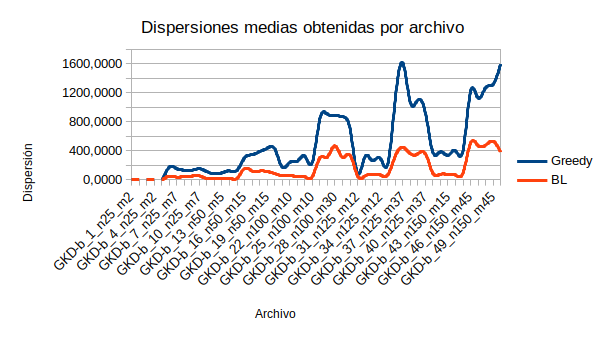
\includegraphics[width=0.45\textwidth]{data/mean_disps.png}
	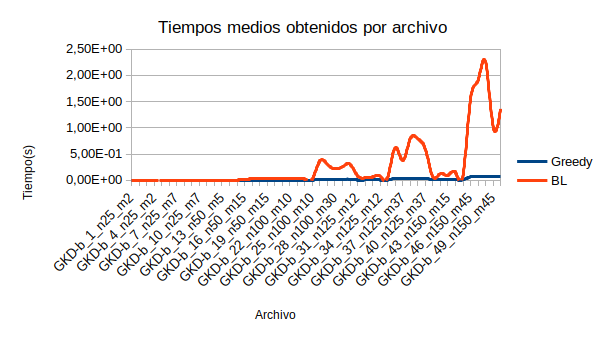
\includegraphics[width=0.45\textwidth]{data/mean_time.png}
	\caption{dispersión y tiempo por archivo}
	\label{fig:dispYTmedios_graf}
\end{figure}

Como observamos, a nivel de dispersión, ambos algoritmos siguen la misma tendencia en todo momento, pero el de búsqueda local se mantiene por debajo del voraz siempre.
En cuanto a tiempos, ambos comienzan de manera similar, pero llega un punto en el que el de búsqueda local sube su tiempo de ejecución. No obstante, este aumento en el tiempo no resulta descabellado si tenemos en cuenta la mejoría en los resultados frente al voraz.

\newpage

\begin{figure}[h]
    \centering
    \begin{minipage}[l]{0.32\textwidth}
	    \begin{tabular}{|c|c|}
	        \hline
	        \textbf{Archivo} & \textbf{Optimo} \\
	        \hline
	        &\\
	        1 & 0\\
            2 & 0\\
            3 & 0\\
            4 & 0\\
            5 & 0\\
            6 & 12,717\\
            7 & 14,098\\
            8 & 16,761\\
            9 & 17,069\\
            10 & 23,26\\
            11 & 1,926\\
            12 & 2,121\\
            13 & 2,362\\
            14 & 1,663\\
            15 & 2,853\\
            16 & 42,74\\
            17 & 48,10\\
            18 & 43,19\\
            19 & 46,41\\
            20 & 47,71\\
            21 & 13,83\\
            22 & 13,66\\
            23 & 15,34\\
            24 & 8,640\\
            25 & 17,20\\
            26 & 168,7\\
            27 & 127,0\\
            28 & 106,3\\
            29 & 137,4\\
            30 & 127,4\\
            31 & 11,74\\
            32 & 18,78\\
            33 & 18,53\\
            34 & 19,48\\
            35 & 18,11\\
            36 & 155,4\\
            37 & 198,8\\
            38 & 187,9\\
            39 & 168,5\\
            40 & 178,1\\
            41 & 23,34\\
            42 & 26,78\\
            43 & 26,75\\
            44 & 25,93\\
            45 & 27,77\\
            46 & 227,7\\
            47 & 228,6\\
            48 & 226,7\\
            49 & 226,4\\
            50 & 248,8\\


	        \hline
	    \end{tabular}
	\end{minipage}
	\begin{minipage}[c]{0.32\textwidth}
	    \begin{tabular}{|c|c|}
	        \hline
	        \multicolumn{2}{|c|}{\textbf{Algoritmo greedy}} \\
	        \hline
	        \textbf{Tiempo} & \textbf{Dispersión} \\
	        \hline
	        8,46E-06 &  0,0000\\ 
            6,85E-06 &  0,0000\\ 
            6,68E-06 &  0,0000\\ 
            6,49E-06 &  0,0000\\ 
            6,73E-06 &  0,0000\\ 
            3,28E-04 &  172,9389\\ 
            3,24E-04 &  151,4784\\ 
            3,27E-04 &  132,5934\\ 
            3,26E-04 &  131,4541\\ 
            3,23E-04 &  151,2385\\ 
            3,46E-04 &  110,6476\\ 
            3,45E-04 &  80,4410\\ 
            3,45E-04 &  93,6333\\ 
            3,45E-04 &  120,3797\\ 
            3,46E-04 &  129,4126\\ 
            2,67E-03 &  302,2888\\ 
            2,69E-03 &  344,0174\\ 
            2,69E-03 &  387,2363\\ 
            2,67E-03 &  432,7591\\ 
            2,67E-03 &  427,7715\\ 
            2,64E-03 &  171,7590\\ 
            2,65E-03 &  240,6561\\ 
            2,69E-03 &  253,9828\\ 
            2,63E-03 &  322,2628\\ 
            2,65E-03 &  238,7843\\ 
            1,97E-02 &  839,3913\\ 
            2,06E-02 &  901,5594\\ 
            2,05E-02 &  889,6144\\ 
            2,10E-02 &  865,4841\\ 
            2,14E-02 &  700,4242\\ 
            4,61E-03 &  86,3618\\ 
            4,79E-03 &  316,8829\\ 
            4,64E-03 &  262,1155\\ 
            4,65E-03 &  298,9516\\ 
            4,80E-03 &  214,9209\\ 
            3,73E-02 &  1094,4853\\ 
            3,72E-02 &  1606,5565\\ 
            3,76E-02 &  1066,3734\\ 
            3,75E-02 &  1097,4133\\ 
            3,73E-02 &  924,1819\\ 
            8,62E-03 &  378,9201\\ 
            8,56E-03 &  383,6978\\ 
            8,65E-03 &  335,2620\\ 
            8,71E-03 &  399,9048\\ 
            8,38E-03 &  405,1055\\ 
            6,52E-02 &  1214,1638\\ 
            6,48E-02 &  1125,7093\\ 
            6,48E-02 &  1265,8778\\ 
            6,43E-02 &  1316,0476\\ 
            6,50E-02 &  1592,4987\\ 
	        \hline
	    \end{tabular}
	\end{minipage}
	\begin{minipage}[c]{0.32\textwidth}
	    \begin{tabular}{|c|c|}
	        \hline
	        \multicolumn{2}{|c|}{\textbf{Algoritmo BL}} \\
	        \hline
	        \textbf{Tiempo} & \textbf{Dispersión} \\
	        \hline
	        3,11E-04 & 0,0000\\
            2,11E-04 & 0,0000\\
            2,11E-04 & 0,0000\\
            2,22E-04 & 0,0000\\
            2,14E-04 & 0,0000\\
            2,46E-03 & 49,0833\\
            2,90E-03 & 34,5253\\
            2,07E-03 & 44,7451\\
            2,66E-03 & 50,3845\\
            2,17E-03 & 52,6371\\
            2,69E-03 & 15,0193\\
            3,28E-03 & 19,5315\\
            2,70E-03 & 14,1592\\
            2,04E-03 & 19,9200\\
            2,42E-03 & 19,0034\\
            1,83E-02 & 154,7710\\
            2,46E-02 & 120,4500\\
            2,91E-02 & 118,8968\\
            2,72E-02 & 113,3795\\
            3,60E-02 & 84,4173\\
            2,48E-02 & 53,7561\\
            2,56E-02 & 59,2516\\
            2,58E-02 & 44,0998\\
            2,24E-02 & 39,4464\\
            2,27E-02 & 42,1936\\
            3,71E-01 & 299,9137\\
            3,01E-01 & 315,1940\\
            2,20E-01 & 465,3706\\
            2,56E-01 & 310,0761\\
            3,02E-01 & 340,4451\\
            8,40E-02 & 51,3877\\
            4,40E-02 & 52,1606\\
            6,05E-02 & 74,9053\\
            7,77E-02 & 66,0790\\
            5,70E-02 & 64,5465\\
            6,23E-01 & 322,4048\\
            3,78E-01 & 448,1244\\
            7,96E-01 & 358,6058\\
            7,91E-01 & 355,2638\\
            5,92E-01 & 359,0492\\
            6,72E-02 & 90,0941\\
            1,25E-01 & 73,7698\\
            9,42E-02 & 74,5123\\
            1,49E-01 & 65,7905\\
            1,01E-01 & 95,5109\\
            1,55E+00 & 503,3408\\
            1,91E+00 & 472,3337\\
            2,25E+00 & 475,1340\\
            1,02E+00 & 530,0055\\
            1,36E+00 & 380,9427\\
	        \hline
	    \end{tabular}
	\end{minipage}
	\caption{Valores medios obtenidos en la ejecución por algoritmo}
	\label{fig:valoresMedios}
\end{figure}

\newpage

Vamos ver ahora los mejores y peores tiempos de ejecución y dispersión obtenidos, para asegurarnos para observar los mejores y peores casos que obtendremos de forma general.

En la figura \ref{fig:valoresLimite} podemos ver los mejores y peores casos de cada algoritmo.

Es destacable que los peores casos del algoritmo de búsqueda local siguen siendo muchísimo mejores que incluso el mejor caso del voraz a nivel de dispersión.

A nivel de tiempo, obviamente gana el voraz, pero, en mi opinión, si esto se tratara de un caso de uso real, sería mucho mejor sacrificar esos segundos en función de obtener un resultado mucho más fiel al óptimo.

Si observamos en la figura \ref{fig:bestVSworseBL} la diferencia de dispersión entre los mejores y peores casos del algoritmo de búsqueda local, podemos ver que por norma general no tienen mucha diferencia y hay algunos casos en los que coinciden.
Esto es buena señal, ya que nos indica que el algoritmo va a tener, de media, buenos resultados si aumentamos el número de casos del problema.

\begin{figure}[H]
    \centering
	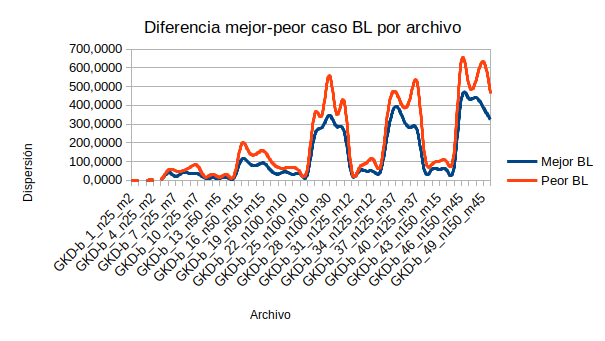
\includegraphics[width=0.8\textwidth]{data/best_vs_worse_bl.png}
	\caption{Diferencia mejor-peor caso por archivo en búsqueda local}
	\label{fig:bestVSworseBL}
\end{figure}

\begin{figure}[h]
    \centering
	\begin{minipage}[l]{0.48\textwidth}
	    \begin{tabular}{|c|c|c|c|}
	        \hline
	        \multicolumn{4}{|c|}{\textbf{Algoritmo greedy}} \\
	        \hline
	        \multicolumn{2}{|c|}{\textbf{Mejores}} & \multicolumn{2}{|c|}{\textbf{Peores}}\\
	        \hline
	        \textbf{Tiempo} & \textbf{Disp} & \textbf{Tiempo} & \textbf{Disp}\\
	        \hline
	        6,31E-06 & 0,0 & 1,41E-05 & 0,0\\
            6,42E-06 & 0,0 & 7,13E-06 & 0,0\\
            6,17E-06 & 0,0 & 6,89E-06 & 0,0\\
            6,11E-06 & 0,0 & 7,26E-06 & 0,0\\
            6,14E-06 & 0,0 & 7,45E-06 & 0,0\\
            3,32E-04 & 114,7 & 3,46E-04 & 298,4\\
            3,28E-04 & 91,2 & 3,99E-04 & 208,1\\
            3,33E-04 & 85,3 & 3,74E-04 & 171,3\\
            3,34E-04 & 73,2 & 3,99E-04 & 213,9\\
            3,37E-04 & 121,9 & 3,46E-04 & 199,7\\
            3,57E-04 & 65,9 & 4,00E-04 & 153,5\\
            3,56E-04 & 47,7 & 3,70E-04 & 107,1\\
            3,51E-04 & 47,6 & 4,11E-04 & 156,5\\
            3,62E-04 & 57,9 & 3,68E-04 & 192,6\\
            3,60E-04 & 88,0 & 3,70E-04 & 168,5\\
            2,75E-03 & 229,6 & 2,82E-03 & 382,4\\
            2,76E-03 & 275,0 & 2,95E-03 & 399,7\\
            2,83E-03 & 316,5 & 2,90E-03 & 451,3\\
            2,75E-03 & 326,7 & 2,94E-03 & 538,8\\
            2,74E-03 & 288,8 & 2,79E-03 & 526,6\\
            2,71E-03 & 109,4 & 2,83E-03 & 266,6\\
            2,76E-03 & 142,7 & 2,85E-03 & 334,9\\
            2,76E-03 & 154,9 & 2,99E-03 & 353,0\\
            2,73E-03 & 259,3 & 2,82E-03 & 356,3\\
            2,79E-03 & 84,2 & 3,16E-03 & 373,1\\
            2,07E-02 & 655,8 & 2,17E-02 & 972,7\\
            2,04E-02 & 731,8 & 2,15E-02 & 1064,3\\
            2,07E-02 & 702,0 & 2,10E-02 & 1310,1\\
            2,08E-02 & 747,2 & 2,20E-02 & 1100,5\\
            2,06E-02 & 576,0 & 2,18E-02 & 798,1\\
            4,90E-03 & 55,7 & 5,06E-03 & 141,4\\
            4,84E-03 & 134,1 & 4,95E-03 & 473,7\\
            4,91E-03 & 197,4 & 5,16E-03 & 427,3\\
            4,87E-03 & 247,8 & 4,93E-03 & 335,2\\
            4,89E-03 & 158,7 & 4,94E-03 & 273,9\\
            3,90E-02 & 901,0 & 4,30E-02 & 1294,5\\
            3,85E-02 & 1463,5 & 3,97E-02 & 1732,8\\
            3,84E-02 & 931,6 & 3,93E-02 & 1447,0\\
            4,00E-02 & 955,9 & 4,07E-02 & 1438,1\\
            3,95E-02 & 828,7 & 4,02E-02 & 1070,7\\
            8,94E-03 & 345,2 & 9,49E-03 & 452,4\\
            9,04E-03 & 329,7 & 9,42E-03 & 434,8\\
            9,01E-03 & 189,9 & 9,88E-03 & 469,2\\
            8,89E-03 & 317,9 & 9,01E-03 & 488,9\\
            9,02E-03 & 321,7 & 9,53E-03 & 497,0\\
            6,87E-02 & 977,1 & 7,20E-02 & 1396,1\\
            6,72E-02 & 991,9 & 6,89E-02 & 1337,8\\
            6,68E-02 & 1187,9 & 6,84E-02 & 1397,1\\
            6,70E-02 & 920,6 & 6,88E-02 & 1575,1\\
            6,73E-02 & 1500,9 & 7,01E-02 & 1829,5\\
	        \hline
	    \end{tabular}
	\end{minipage}
	\begin{minipage}[r]{0.48\textwidth}
	    \begin{tabular}{|c|c|c|c|}
	        \hline
	        \multicolumn{4}{|c|}{\textbf{Algoritmo BL}} \\
	        \hline
	        \multicolumn{2}{|c|}{\textbf{Mejores}} & \multicolumn{2}{|c|}{\textbf{Peores}}\\
	        \hline
	        \textbf{Tiempo} & \textbf{Disp} & \textbf{Tiempo} & \textbf{Disp}\\
	        \hline
	        1,63E-04 & 0,0 & 8,95E-04 & 0,0\\
            2,05E-04 & 0,0 & 2,19E-04 & 0,0\\
            2,07E-04 & 0,0 & 2,18E-04 & 0,0\\
            2,09E-04 & 0,0 & 2,63E-04 & 0,0\\
            2,12E-04 & 0,0 & 2,18E-04 & 0,0\\
            1,77E-03 & 40,8 & 4,14E-03 & 54,4\\
            1,41E-03 & 20,8 & 3,72E-03 & 50,4\\
            1,81E-03 & 40,0 & 2,36E-03 & 50,8\\
            1,22E-03 & 35,9 & 4,79E-03 & 70,8\\
            1,41E-03 & 35,1 & 3,24E-03 & 76,4\\
            1,96E-03 & 12,1 & 3,67E-03 & 17,7\\
            1,88E-03 & 12,7 & 5,10E-03 & 32,9\\
            2,02E-03 & 10,7 & 3,32E-03 & 16,2\\
            1,30E-03 & 14,7 & 3,39E-03 & 29,7\\
            1,59E-03 & 13,8 & 3,80E-03 & 26,8\\
            1,05E-02 & 110,1 & 3,53E-02 & 191,4\\
            1,07E-02 & 93,1 & 5,17E-02 & 152,7\\
            9,72E-03 & 79,2 & 4,40E-02 & 139,1\\
            1,58E-02 & 91,7 & 3,71E-02 & 157,0\\
            2,10E-02 & 52,3 & 5,01E-02 & 103,2\\
            1,23E-02 & 33,2 & 4,39E-02 & 68,5\\
            2,02E-02 & 45,5 & 3,19E-02 & 65,3\\
            1,23E-02 & 31,6 & 4,15E-02 & 70,2\\
            1,17E-02 & 33,7 & 3,99E-02 & 42,2\\
            1,07E-02 & 31,7 & 3,77E-02 & 63,5\\
            1,87E-01 & 240,7 & 9,01E-01 & 354,8\\
            1,29E-01 & 280,9 & 4,86E-01 & 351,2\\
            6,72E-02 & 346,8 & 6,27E-01 & 560,0\\
            1,29E-01 & 285,7 & 3,90E-01 & 351,4\\
            2,09E-01 & 260,0 & 4,29E-01 & 421,3\\
            2,31E-02 & 37,4 & 1,59E-01 & 62,6\\
            2,33E-02 & 47,3 & 5,95E-02 & 60,7\\
            2,40E-02 & 49,2 & 1,06E-01 & 92,0\\
            5,02E-02 & 46,3 & 1,03E-01 & 109,3\\
            2,86E-02 & 53,0 & 9,05E-02 & 79,7\\
            2,69E-01 & 260,2 & 1,59E+00 & 373,2\\
            1,79E-01 & 393,9 & 5,70E-01 & 472,8\\
            2,01E-01 & 332,4 & 2,23E+00 & 393,9\\
            1,79E-01 & 281,7 & 1,24E+00 & 437,7\\
            1,94E-01 & 260,9 & 9,09E-01 & 514,6\\
            3,45E-02 & 48,5 & 1,13E-01 & 135,1\\
            8,57E-02 & 59,4 & 1,56E-01 & 86,2\\
            3,92E-02 & 58,5 & 1,60E-01 & 101,9\\
            4,97E-02 & 53,9 & 2,45E-01 & 99,4\\
            6,15E-02 & 68,5 & 1,68E-01 & 149,6\\
            7,65E-01 & 431,3 & 2,59E+00 & 634,2\\
            6,11E-01 & 438,3 & 4,40E+00 & 515,3\\
            8,71E-01 & 441,2 & 3,24E+00 & 533,7\\
            7,12E-01 & 387,9 & 1,43E+00 & 632,7\\
            2,35E-01 & 322,4 & 2,35E+00 & 462,4\\
	        \hline
	    \end{tabular}
	\end{minipage}
	\caption{Mejores y peores valores obtenidos por algoritmo}
	\label{fig:valoresLimite}
\end{figure}













\end{document}